% !TeX root = ../main.tex

\section{Marco conceptual}
\label{sec:marco-conceptual}

\subsection{Componentes y notación del sistema}
\label{subsec:componentes-cola}

Un sistema de colas se describe mediante las entidades que requieren atención, el proceso de llegadas, el espacio de espera y los recursos que prestan el servicio. En este trabajo, una entidad representa una solicitud o trabajo, sin asociarla a una organización concreta. La llegada marca su ingreso al sistema; si el servidor está libre, comienza la atención inmediatamente. En caso contrario, la entidad permanece en la cola hasta que puede ser atendida. La salida ocurre al finalizar el servicio. Por tanto, la cola comprende únicamente las entidades que esperan, mientras que el sistema incluye también a la que está recibiendo atención.

La figura~\ref{fig:cola-un-servidor} separa estos componentes para evitar confundir acumulación y atención. El bloque de espera representa una capacidad ilimitada, no una cantidad fija de lugares. La secuencia muestra el recorrido lógico: pasar por la cola no implica una espera positiva cuando el servidor está disponible.

\begin{figure}[htbp]
  \centering
  % Fragmento editable. Requiere tikz; no requiere bibliotecas adicionales.
% Esquema de componentes: no representa una realización ni un número de clientes.
% Ancho nominal: 0.96\textwidth, incluidos los bloques extremos.
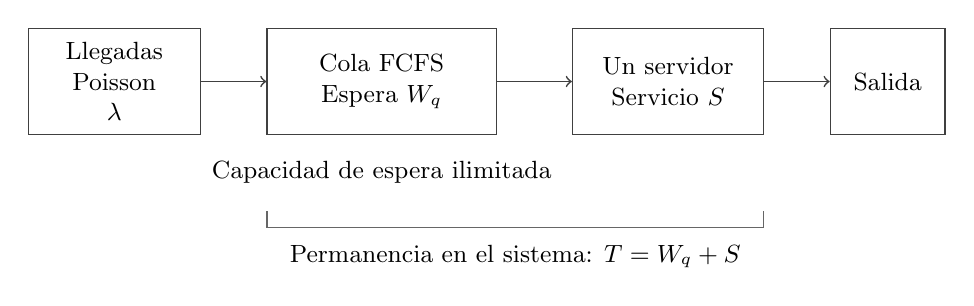
\begin{tikzpicture}[
  x=\textwidth,y=1cm,font=\small,
  bloque/.style={draw=black!75,fill=white,line width=0.5pt,
    align=center,inner sep=0pt,minimum height=1.35cm},
  flujo/.style={->,draw=black!75,line width=0.6pt}
]
  \node[bloque,text width=0.18\textwidth] (llegadas) at (0.09,0)
    {Llegadas\\Poisson\\$\lambda$};
  \node[bloque,text width=0.24\textwidth] (cola) at (0.37,0)
    {Cola FCFS\\Espera $W_q$};
  \node[bloque,text width=0.20\textwidth] (servidor) at (0.67,0)
    {Un servidor\\Servicio $S$};
  \node[bloque,text width=0.12\textwidth] (salida) at (0.90,0)
    {Salida};
  \draw[flujo] (llegadas.east) -- (cola.west);
  \draw[flujo] (cola.east) -- (servidor.west);
  \draw[flujo] (servidor.east) -- (salida.west);
  \node[align=center] at (0.37,-1.15) {Capacidad de espera ilimitada};
  \draw[draw=black!60,line width=0.45pt]
    (0.25,-1.65) -- (0.25,-1.85) -- (0.77,-1.85) -- (0.77,-1.65);
  \node[align=center,anchor=north] at (0.51,-1.95)
    {Permanencia en el sistema: $T=W_q+S$};
\end{tikzpicture}

  \caption{Esquema conceptual de una cola M/G/1 con disciplina FCFS. Elaboración propia basada en la descripción del modelo de Virtamo \cite{virtamoMG1}. Los bloques representan componentes, no cantidades observadas de entidades.}
  \label{fig:cola-un-servidor}
\end{figure}

La notación de Kendall, en su forma abreviada $A/S/c$, resume el proceso de llegadas, la distribución de los tiempos de servicio y el número de servidores. En esta expresión, $S$ ocupa una posición descriptiva; más adelante se utilizará también como símbolo de la variable aleatoria de servicio. La letra M identifica el caso sin memoria: llegadas Poisson en la primera posición y servicio exponencial en la segunda. D indica una duración determinista y G una distribución general. Así, M/G/1 describe llegadas Poisson, servicio general y un solo servidor \cite{virtamoMG1}. La abreviatura no reemplaza la especificación de la capacidad de espera ni de la disciplina de atención, que deben declararse por separado.

En particular, M/D/1 y M/M/1 son casos de la familia M/G/1: el primero fija una duración constante del servicio y el segundo adopta una distribución exponencial. La letra G no designa una tercera distribución elegida para comparar, sino que permite analizar distintas distribuciones mediante un marco común. Una distribución adicional para la futura demostración requerirá una elección y una parametrización explícitas en la metodología.

\subsection{Llegadas, servicio y disciplina de atención}
\label{subsec:llegadas-servicio-fcfs}

Se supone un proceso de Poisson homogéneo de tasa $\lambda>0$. Esto significa que el número de llegadas en un intervalo de duración $t$ tiene distribución Poisson de media $\lambda t$ y que los conteos en intervalos disjuntos son independientes. Los tiempos entre llegadas consecutivas son independientes y tienen distribución exponencial de parámetro $\lambda$, con media $1/\lambda$. La tasa se expresa en entidades por unidad de tiempo. Su constancia describe la intensidad media de la demanda, pero no implica que las llegadas estén igualmente espaciadas.

El tiempo de servicio se representa mediante una variable aleatoria no negativa $S$. Las duraciones de las sucesivas atenciones son independientes e idénticamente distribuidas e independientes del proceso de llegadas. Se adopta FCFS, del inglés \emph{first-come, first-served}: las entidades comienzan a ser atendidas en el orden en que llegan. El servicio es no expropiativo, es decir, una atención iniciada no se interrumpe para atender otra solicitud. Además, el servidor trabaja siempre que hay entidades pendientes; no se incluyen pausas, vacaciones ni tiempos adicionales de preparación.

Se considera una fuente potencial infinita, por lo que la intensidad de llegada no disminuye por la cantidad de entidades dentro del sistema. La capacidad de espera es ilimitada y no hay rechazos ni abandonos: toda llegada permanece hasta completar su atención. Estos supuestos permiten usar la misma tasa $\lambda$ para los ingresos y, en régimen estacionario, para las salidas. El marco corresponde a una cola abierta aislada, no a una red cerrada ni a un modelo con prioridades.

\subsection{Media, variabilidad y utilización}
\label{subsec:variabilidad-utilizacion}

La media del servicio y su tasa media equivalente se definen como
\begin{equation}
  m=\mathrm{E}[S], \qquad \mu=\frac{1}{m}, \qquad 0<m<\infty.
  \label{eq:media-tasa-servicio}
\end{equation}
Si $m$ se mide en minutos por entidad, $\mu$ se expresa en entidades por minuto. Definir $\mu$ como el inverso de la media no presupone que el servicio sea exponencial. La dispersión de las duraciones se caracteriza mediante
\begin{equation}
  \operatorname{Var}(S)=\mathrm{E}[(S-m)^2],
  \qquad C_s^2=\frac{\operatorname{Var}(S)}{m^2}.
  \label{eq:variabilidad-servicio}
\end{equation}
La varianza tiene unidades de tiempo al cuadrado. El coeficiente de variación $C_s=\sqrt{\operatorname{Var}(S)}/m$ y su cuadrado $C_s^2$ son adimensionales; este último permite expresar la dispersión relativa sin depender de la unidad temporal. El segundo momento satisface
\begin{equation}
  \mathrm{E}[S^2]=\operatorname{Var}(S)+m^2=m^2(1+C_s^2).
  \label{eq:segundo-momento-servicio}
\end{equation}
Estas relaciones permiten separar el nivel medio de atención de su variabilidad \cite{virtamoMG1}.

La intensidad de tráfico es
\begin{equation}
  \rho=\lambda m=\frac{\lambda}{\mu}<1.
  \label{eq:utilizacion-estabilidad}
\end{equation}
Es una cantidad adimensional y, bajo los supuestos adoptados en régimen estacionario, representa la fracción de tiempo que el servidor permanece ocupado. La desigualdad establece la condición de estabilidad: el trabajo que ingresa por unidad de tiempo debe ser inferior a la capacidad disponible \cite{virtamoMG1}. No significa que nunca se formen colas; aun con capacidad media suficiente, la irregularidad de llegadas y servicios produce esperas. Para estudiar una espera media finita se exige además $\mathrm{E}[S^2]<\infty$. Estabilidad y finitud de ese promedio son requisitos distintos: una media de servicio finita no garantiza un segundo momento finito.

\subsection{Medidas de desempeño y ley de Little}
\label{subsec:medidas-little}

Se denota por $W_q$ el tiempo aleatorio que una entidad espera antes de iniciar su atención, y por $T$ su tiempo total en el sistema. Para esa misma entidad,
\begin{equation}
  T=W_q+S, \qquad \mathrm{E}[T]=\mathrm{E}[W_q]+m.
  \label{eq:tiempo-sistema}
\end{equation}
El subíndice $q$ identifica la espera en cola. Esta distinción evita atribuir al servicio propio una demora que corresponde a trabajos anteriores. Una entidad atendida inmediatamente tiene $W_q=0$, aunque su permanencia total incluya el servicio.

Sean $N_q$ y $N$ las cantidades aleatorias de entidades en espera y en el sistema, respectivamente, observadas en régimen estacionario. Sus medias se escriben $L_q=\mathrm{E}[N_q]$ y $L=\mathrm{E}[N]$. La ley de Little relaciona estas cantidades con los tiempos medios:
\begin{equation}
  L_q=\lambda\mathrm{E}[W_q], \qquad L=\lambda\mathrm{E}[T].
  \label{eq:ley-little}
\end{equation}
Se aplica aquí en condiciones estacionarias, con tasas de flujo coherentes y promedios finitos \cite{virtamoMG1}. No es una igualdad entre observaciones individuales ni una garantía de coincidencia exacta en una ejecución finita. Tampoco requiere por sí misma distribuciones Poisson o exponenciales: su generalidad es mayor que la del modelo empleado para calcular la espera. En este sistema, las ecuaciones anteriores implican $L=L_q+\rho$, pues a las entidades que esperan se suma la ocupación media del único servidor.

\subsection{Fórmula de Pollaczek--Khinchine e interpretación}
\label{subsec:pollaczek-khinchine}

Para una cola M/G/1 FCFS con los supuestos anteriores, la fórmula de Pollaczek--Khinchine establece
\begin{equation}
  \mathrm{E}[W_q]
  =\frac{\lambda\mathrm{E}[S^2]}{2(1-\rho)}
  =\frac{\rho m(1+C_s^2)}{2(1-\rho)}.
  \label{eq:pollaczek-khinchine}
\end{equation}
Virtamo desarrolla esta relación a partir del servicio residual y de la cantidad de entidades por delante de una llegada \cite{virtamoMG1}. Ambas expresiones tienen unidades de tiempo y describen una media estacionaria, no la espera de cada entidad.

La interpretación del servicio residual explica por qué interviene el segundo momento. Una llegada que encuentra ocupado al servidor debe esperar el resto de la atención en curso, además del servicio de quienes ya están en cola. Los servicios prolongados ocupan una mayor parte del tiempo y, por ello, tienen más probabilidad de ser encontrados por una observación temporal que los breves. No corresponde suponer que el servicio encontrado es una selección uniforme entre todas las atenciones. Las llegadas Poisson observan las proporciones temporales del estado del sistema, propiedad conocida como PASTA \cite{virtamoMG1}.

Si $R$ es el servicio residual observado, definido como cero cuando el servidor está libre, entonces
\begin{equation}
  \mathrm{E}[R]=\frac{\lambda\mathrm{E}[S^2]}{2},
  \qquad
  \mathrm{E}[W_q]=L_q m+\mathrm{E}[R].
  \label{eq:servicio-residual}
\end{equation}
Al sustituir Little y despejar se obtiene la ecuación~\ref{eq:pollaczek-khinchine}. Condicionado a encontrar ocupado al servidor, el residual medio es $\mathrm{E}[S^2]/(2m)$, no en general $m/2$. Esta diferencia recoge el mayor peso temporal de los servicios largos; incluso el servicio constante deja una espera residual cuando una llegada ocurre durante su ejecución.

Con $\lambda$ y $m$ fijos, también queda fija $\rho$. La espera media aumenta linealmente con la varianza del servicio, mientras que el factor $1/(1-\rho)$ amplifica la congestión al acercarse la utilización a uno. Dos distribuciones con iguales primeros dos momentos producen la misma espera media dentro de este modelo \cite{virtamoMG1}; no se deduce que tengan iguales distribuciones de espera, percentiles o probabilidades de demoras extremas.

\subsection{Casos particulares y alcance de la comparación}
\label{subsec:comparacion-casos}

El servicio determinista tiene $S=m$ y varianza nula; el exponencial de media $m$ tiene varianza $m^2$. Su sustitución en Pollaczek--Khinchine proporciona la comparación simbólica de la tabla~\ref{tab:casos-servicio}, manteniendo iguales $\lambda$ y $m$ \cite{virtamoMG1}.

\begin{table}[htbp]
  \centering
  \caption{Espera media teórica para dos casos de M/G/1 FCFS, con igual tasa de llegada y media de servicio.}
  \label{tab:casos-servicio}
  \begin{tabular}{lccc}
    \hline
    Modelo & Servicio & $C_s^2$ & $\mathrm{E}[W_q]$ \\
    \hline
    M/D/1 & Constante & $0$ & $\displaystyle\frac{\rho m}{2(1-\rho)}$ \\[6pt]
    M/M/1 & Exponencial & $1$ & $\displaystyle\frac{\rho m}{1-\rho}$ \\[6pt]
    \hline
  \end{tabular}
\end{table}

Bajo estas condiciones, la espera media con servicio exponencial es el doble de la correspondiente al servicio constante. La relación no se traslada directamente al tiempo total, porque ambos casos añaden la misma media $m$ de servicio propio. Además, como la varianza no puede ser negativa, el caso determinista minimiza la espera media entre las distribuciones admisibles de igual media. Son consecuencias analíticas del modelo, no hallazgos experimentales de esta monografía.

Este marco fija el lenguaje de la comparación posterior. La demostración prevista en Python, mediante un notebook compatible con Google Colab, deberá distinguir las identidades teóricas de las estimaciones obtenidas en ejecuciones finitas y considerar su incertidumbre. Aquí no se presentan simulaciones ejecutadas ni validación de un servicio real. La elección de una tercera distribución y el diseño de las réplicas corresponden a la metodología; las conclusiones sobre otras disciplinas o métricas exigirán evidencia específica.
